\section{Discovering stellar variability \label{sec:intro-stellar-variability}}

\intent{Ancient observations}

It is undeniable that ancient civilizations looked to the night sky with great interest. 
Stars were considered immovable and immutable, with the notable exceptions of planets and Nov\ae{}.
But periodic stellar variability was probably known since antiquity too.
For instance, Egyptians knew the period of Algol three millennia ago \citep{Jetsu2013,Jetsu2015},
and the mythology of several cultures seems to have some references to the phenomenon \citep{Wilk1996}. 
On some cases, periodic variable stars were recorded as Nov\ae{} by ancient eastern cultures \citep{HOPENGYOKE1962}.

\intent{Western rediscovery}

The modern rediscovery of stars having periodic changes on their brightness is accredited to Fabricius, 
who discovered Mira ($o$ Ceti) in 1596 \citep{Hoffleit1997}.
This phenomenon was in direct contradiction with the classical philosophical view of the Universe, as expressed by \citet[book I, part 3]{aristotle}: 
\enquote{so far as our inherited records reach, no change appears to have taken place either in the whole scheme of the outermost heaven or in any of its proper parts}.
On the following centuries several other stars were marked as candidates for periodic variables.
Edward Pigott and his collaborator John Goodricke were verifying those candidates in 1784 \citep{Hoskin1979}. 
Famously, \cite{Pigott1785} observed $\eta$ Aquil\ae{} and confirmed its variability, 
while \cite{Goodricke1786} observed $\delta$ Cephei, Algol, $\beta$ Lyr\ae{}, and other stars.


\intent{Initial theories for stellar variability}

Pigott and Goodricke results are remarkable, as almost a century would pass until the formalization of the magnitude scale for brightness by \cite{Pogson1856}.
But despite the lack of truly (instrumental) quantitative measurements of brightness, 
there were plenty of theories regarding the mechanism behind stellar variability. 
Those theories included planetary eclipses, star-star collisions, binary stars, meteor impacts, 
darkening by gas or dust clouds, and sun-like spots coupled with rotation and axial tilts \citep{Hoffleit1993}. 
And although the eclipse conjecture was later proved to be the correct for Algol \citep{Pickering1880}, 
the asymmetric behavior of the brightness of some stars (as those seen in \autoref{fig:first-cepheids}) could not be accounted for.
If the change of brightness were to be the product of an eclipse,
the brightness would spend the same amount of time increasing as decreasing,
as the transiting object covers and uncovers the star.
On the same train of thought, if the star happened to have a side full of spots, or obscured by a dust cloud,
no stable movement could make the brightness go from minimum to maximum faster than from maximum to minimum on such a periodic manner.

\begin{figure}[H] 
	\centering
	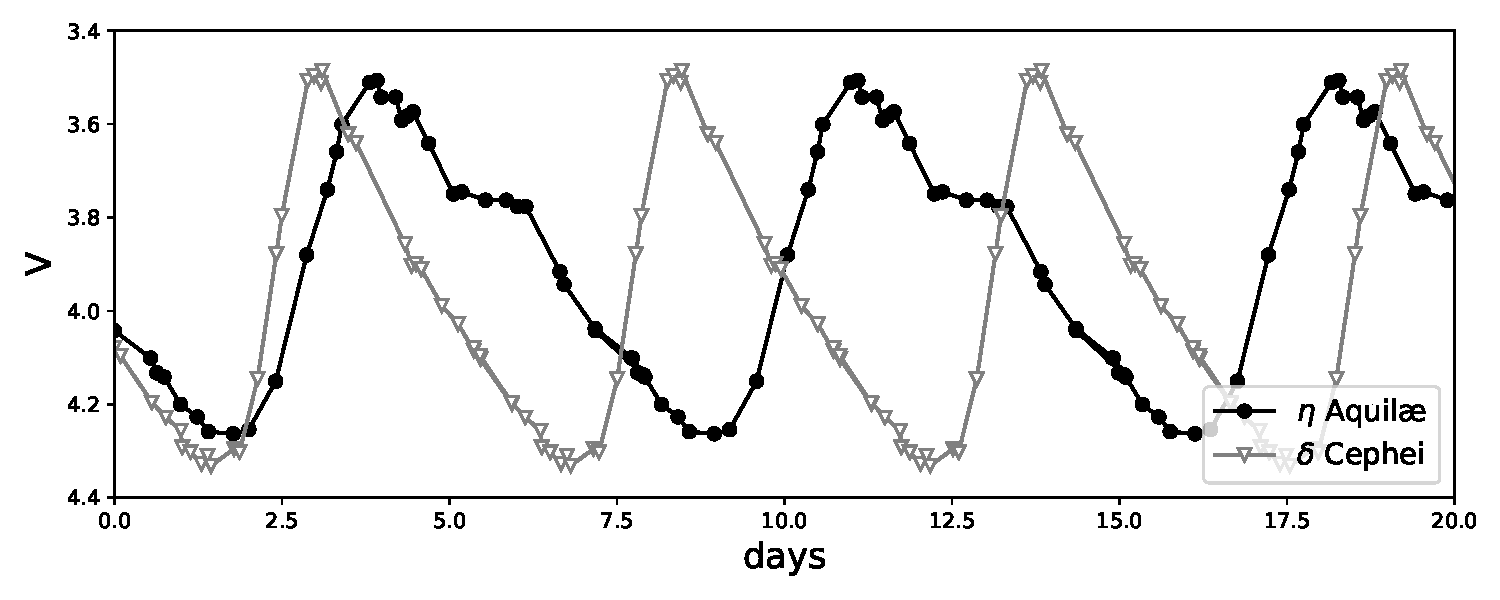
\includegraphics[width=0.9\textwidth]{img/eta_aquilae_delta_cephei_light_curves.pdf}
	\caption[Light curve of $\delta$ Cephei and $\eta$ Aquilæ]{Modern light curves for the first two discovered Cepheid variable stars. 
	$\eta$ Aquil\ae{} has a period of $\sim7.17$ days, in contrast with the $\sim5.36$ days of $\delta$ Cephei.
	Objects are brighter as magnitude (V) decreases (see chapter 2 for details). 
	Note how both stars take more time decreasing their brightness than increasing it. 
	Figure reconstructed from \cite{Kiss1998} data.}
	\label{fig:first-cepheids}
\end{figure}

\section{The birth of the Period-Luminosity relation}

\intent{The need of classification }

These variable stars were initially classified by \cite{Pickering1880}, only taking into account the shape of the light curve: 
Nov\ae{}, Mira-like, eclipsing, irregular variables, and class for the aforementioned irregular (but highly periodic) case, namely $\beta$ Lyr\ae{} and $\delta$ Cephei.
There was a need for further classification of these stars, with several attempts of break down Pickering classes \citep{Lockyer1896,Lockyer1897}, 
but it would take several important discoveries in astronomy for the classification of variable stars to fully develop,
resulting in $\delta$ Cephei as the prototype of its own class of variable stars.
% log day units in caption

\intent{Work and discoveries of the Harvard Computers}

\begin{figure}
	\centering
	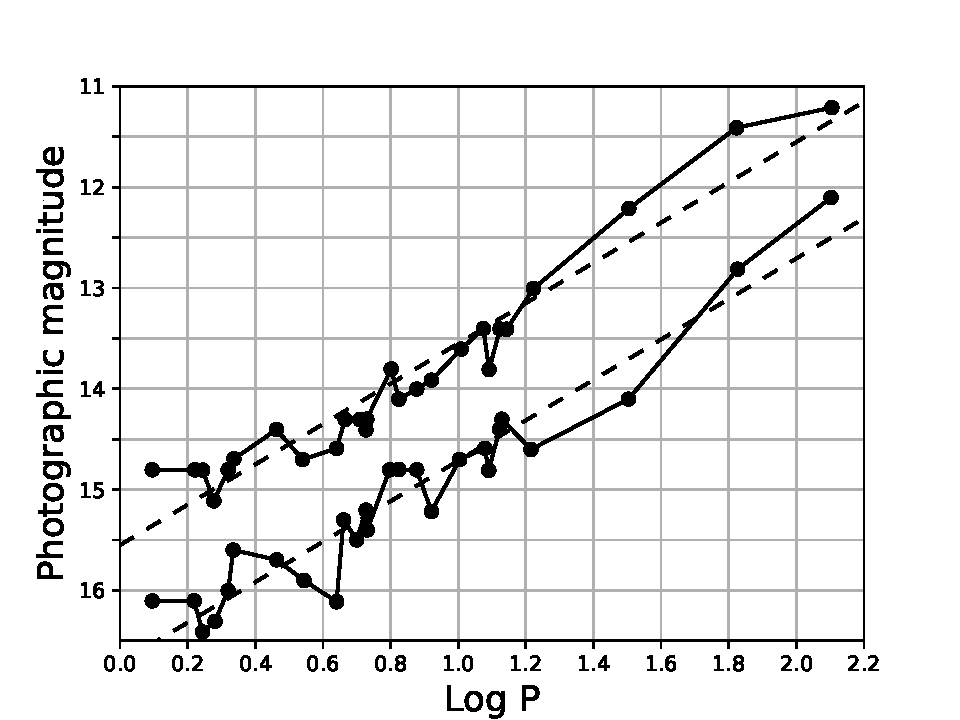
\includegraphics[width=0.7\textwidth]{img/leavitt.pdf}
	\caption[Leavitt PL relation]{\cite{Leavitt1912} representation of the relationship between period and luminosity 
	of 25 Cepheid stars in the Small Magellanic Cloud.
	The two data series refer to the points of maximum and minimum brightness for each star. 
	The period of the stars ($P$) is reported on days, so the abscissa is in units of $\log(\text{days})$.
	The ordinate is given in photographic magnitude.
	}
	\label{fig:leavitt}
\end{figure}

Those next big steps on the field were done by Pickering's ``computers'' women at Harvard. 
Although the universities refused to let women study at the time, Pickering (then director of Harvard College Observatory) 
needed people to process and analyze the sheer amount of data being produced in the observatory, 
on the form of stellar spectra and photographic plates of the observations.
Working there, Williamina Fleming prepared the Draper Catalog of stellar spectra \citep{Pickering1890,Maury1897}, 
which allowed her to classify Mira-type stars and Nov\ae{} with only their spectrum. 
This classification system was later reordered by \cite{Canon1901} to reflect the temperature of the stars.
Around that time Henrietta Leavitt joined the Harvard computers, 
with the task of searching for variable stars in the Magellanic Clouds, satellite galaxies of the Milky Way known as the time as Nebul\ae{}.
There she discovered almost two thousand variables \citep{Leavitt1908}, around seven hundred of this variables belong to the Cepheid class. 
By calculating the periods of 25 of those stars and comparing them to their maximum and minimum magnitudes, Leavitt found a linear relationship (\autoref{fig:leavitt}).

\intent{The Period-Luminosity relation}

Leavitt's discovery was of immense importance as a possible tool for measuring the distance to the farthest Cepheid stars. 
She noted: \enquote{Since the variables are probably at nearly the same distance from the Earth,
their periods are apparently associated with their actual emission of light} \citep[page 3]{Leavitt1912}.
Leavitt knew she was seeing the \textit{apparent} brightness of the stars, as brightness decreases with distance.
If distances to near Cepheids could be found by another method, 
this Period-Luminosity (PL) relation could be reversed to find the \textit{absolute} brightness of the Cepheids in the Small Magellanic Cloud (SMC),
finding the distance to the Nebula.
Leavitt correctly proposed the method of parallaxes to solve this task, but his work on Harvard did not let her pursue this investigation.

\intent{fine-tuning the PR relation and the Magellanic Clouds}

The parallaxes for the nearest Cepheids were examined by \cite{Hertzsprung1913}.
He used Leavitt's PL relation to calculate the distance to the SMC, 
giving \citep[after a \enquote{pen error}, see][]{Fernie1969} 9.2 kilo parsecs (kpc) (equivalent to 30 kly), which is a vast underestimation.
\cite{Shapley1918} improved further the precision of Leavitt's original PL relation, 
but its zero point (its accuracy) was assumed to be the correct one, despite having several systematic and selection errors \citep{Fernie1969}.
Shapley used his results to calculate the distance to the Magellanic Clouds, 
obtaining 32.5 kpc (106 kly) for the Small Cloud \citep{Shapley1924S} and 34.4 kpc (112 kly) for the Large Cloud \citep{Shapley1924L}.

\section{Measuring space and time with variable stars}

\intent{The great debate, and Hubble measuring the size of the Universe}

Around this time, there was a big debate in the astronomical community around the nature of the so-called \enquote{spiral Nebul\ae{}}.
Were those Nebul\ae{} part of the Milky Way, or were they their own separate, distant galaxies?
E. Hubble, using Shapley's version of the PL relation, settled the matter when he found a distance of 285 kpc (929 kly) for M31 and M33 
\citep[now called the Andromeda and Triangulum galaxies,][]{Hubble1925a}
and 214 (697 kly) for NGC 6822 \citep[Barnard's galaxy,][]{Hubble1925b}, 
surpassing Shapley's hypothesis that the Galaxy (and the whole Universe) was only 92 kpc (300 kly) wide \citep{ShapleyCurtis1921}.

\intent{Space means time: the Cosmic age problem}

With this results, \cite{Hubble1929} measured the redshift of some extra-galactic Nebul\ae{}, 
and encountered a linear relationship between distance and velocity.
It was the first experimental evidence of the general relativity prediction of an expanding Universe \citep{Fiedmann1922,Lemaitre1927}.
Hubble estimate of this expanding rate was $H_0 \approx 550 (\text{km}/\text{s})/\text{Mpc}$ (the Hubble's constant), 
which implied the Universe must have an age of $~2\times10^9$ years. 
Meanwhile, geologists estimated the age of the Earth as $~4\times10^9$ years \citep[for an historical account see]{Dalrymple1994}.
How could be the Earth older than the Universe? There was a big problem in the figures, somewhere.

\intent{Baade correction}

Hubble, again, had half the answer. He had some concerns about the zero point of Shapley's PL relation, 
an opinion shared with \cite{Baade1944} after he divided the stars on two populations based on their metallicities.
Baade realized that population I Cepheids were 1.5 magnitudes brighter than population II (for the same period) 
so there were \textit{two} different PL relations, shifted on their zero point by 1.5 magnitudes.
He proved his hypothesis at Palomar Observatory, observing the Andromeda nebula \citep{Baade1956,Arp1955}.
As a consequence of the distance-modulus equation, measurements made with population I Cepheids should be scaled by a factor of $10^{3/10}\approx 2$.
The Hubble distances were based on population I Cepheids, and  therefore his distances doubled
\footnote{Shaple's distance to the SMC was a little more than its actual value of $\sim 60$ kpc, so this doubling actually made his results very accurate for his time.}. 
This resulted on a halved Hubble constant and consequently doubled the observed age of the Universe, $\sim1.7\times 10^9$ years.
\cite{Patterson1955} measured the age of the Earth as $4.55\times10^9$ years, so the problem was not solved yet.

\intent{Sandage correction}

A second correction came from the work of Sandage. 
First reviewing Hubble's work with more data \citep{Sandage1956}, and then correcting another problem:
Hubble had made the calibration of the distance for the farthest nebul\ae{} with the brightest resolvable stars he had,
possible incurring in an identification mistakes with ionized Hydrogen regions or multiple nearby stars \citep{Sandage1958}.
This considerations amounted a total correction of 4.1 magnitudes, 
and produced a Hubble's constant of $H_0 \approx 75 (\text{km}/\text{s})/\text{Mpc}$, 
or a timescale for the Universe of $\sim1.3\times 10^{10}$ years, comparable to modern estimates \citep{Freedman2001}.

\section{Recent developments}

\intent{Present status of the distance ladder}

In the present day, mainly two astronomical projects are entitled to the search of variable stars and the refinement of cosmic distances estimation:
the OGLE project\footnote{\url{http://ogle.astrouw.edu.pl/}} and the Araucaria project\footnote{\url{https://araucaria.camk.edu.pl/}}.
While the Gaia space observatory measures parallaxes, the first step on the distance ladder, 
the OGLE project surveys the Galaxy and the Magellanic Clouds in search of variable stars and gravitational microlensing.
They have nearly completed Leavitt initial task of catalogue the Cepheid stars on the Magellanic Clouds \citep{OGLE2017},
and their survey of Cepheids on the Milky Way has allowed to further study its structure \citep{Skowron2019} and its dynamics \citep{Mroz2019}.
On the other side, the Araucaria project focuses on the calibration of standard candles, comparing different methods: 
they have calibrated the distance to the SMC within a 3\% of precision \citep{Araucaria2014} and to the LMC within a 1\% \citep{Araucaria2019}.


\intent{The other spectrum, the Fourier spectrum}

Just one more particular problem has surfaced on the PL relation. 
As a consequence of the pulsation mechanism of these stars, 
the underlying physical machinery that makes their brightness oscillate,
Cepheid variable stars can pulsate on several \textit{overtones} of their natural frequency.
This overtones displaces the PL relation, as is multiplicative operation on the period, 
which amounts on a different position on the $\log P$ axis.
Therefore, stars with different modes of pulsation must be separated before attempting to calibrate a PL relation \citep{Zabolotski2005}.
The most natural way of attacking this problem is using the other spectrum of the star: 
not the light-energy usual spectrum, but the Fourier spectrum, 
which allows us to see the frequencies and phase properties of the light curve.

We have seen that as experimental techniques evolve and become more precise, 
the theoretical aspects of the PL relation became increasingly important for the accurate determination of distances on the Universe.
Even so, with the amount of observational data these projects are producing, 
the use of efficient and robust methods for analyzing it became imperative too.

Although of capital importance, the methods of image reduction and magnitude determination lie outside the scope of this work.
The aim of this monograph is to examine and implement the different methods for finding the period of populations of Cepheids in the Magellanic Clouds.
Each method will be tested on real Cepheid data, in order to select the one better suited for the task of producing reliable PL relations.
The resulting method will be used to replicate the PL relations of the Cepheids on the Magellanic Clouds given by \cite{OGLE2016}.



